\documentclass[12pt]{article}

\usepackage{graphicx}
\usepackage{geometry}
\usepackage{setspace}
\usepackage{multirow}
\usepackage[table,xcdraw]{xcolor}
\usepackage{caption}
\geometry{a4paper, total={170mm, 257mm}, left=20mm, right=20mm, top=25mm, bottom=25mm}


\usepackage{fancyhdr}
\pagestyle{fancy}
\fancyhf{} % Limpia los estilos anteriores de encabezado y pie de página

% Define el contenido del encabezado
\rhead{Tecnológico de Costa Rica}

% Opcional: Puedes personalizar el pie de página si lo necesitas
% \lfoot{Pie de página izquierdo}
\cfoot{\thepage} % Número de página en el centro
% \rfoot{Pie de página derecho}

% Línea horizontal en la parte superior del encabezado
\renewcommand{\headrulewidth}{0.5pt}

\setlength{\parindent}{1em}
\setlength{\parskip}{1em}

\usepackage{makeidx}
\makeindex


%%%%%%%%%%%%%%%%%%%%%%%%%%%%%%%%%%%%%%%%%%%%%%%%%%%%%%%%%%%%%%%%%%%%%%%%%%%%%%%%%%%%%%%%%%%%%%%%%%%%%%%%%%%%%%%%%%%%%% here Begins the document

\begin{document}
\begin{titlepage}

\centering


\vspace{10cm}

\textbf{\LARGE Instituto Tecnológico de Costa Rica}

\vspace{2cm}

\textbf{\LARGE Escuela de Ingeniería Electrónica}

\vspace{2cm}


\includegraphics[width=10cm]{logotec/image.png}
\vspace{2cm}

\hrule

\vspace{1cm}

\textbf{\LARGE Diseño e implementación de un software agnóstico de hardware para la manipulación de un sistema de control para el  comportamiento dinámico de una planta prototipo de control automático}

\vspace{1cm}

\hrule

\vspace{1cm}

\textbf{\LARGE SIPLab-TEC}

\vspace{1cm}

\textbf{\LARGE David Felipe Duarte Sanchez}

\vspace{1cm}

\textbf{\LARGE 2017239606}

\vspace{1cm}

\today % Esto agrega la fecha actual

\end{titlepage}
.
\par
\vspace{16cm} % Ajusta la cantidad de espacio vertical según sea necesario

Yo, David Duarte Sanchez portador de la cédula 305070982, declaro que los resultados obtenidos en el presente trabajo de investigación, previo a la obtención del titulo de Licenciado en Ingenierıa en Electrónica, son absolutamente originales, auténticos y personales.

Soy consciente de que el hecho de no respetar los derechos de autor y realizar una mala conducta científica; es decir, fabricación de datos falsos y plagio, conlleva
sanciones universitarias y/o legales.

En tal virtud, declaro que el trabajo de investigación realizado sujeto a evaluación no ha sido presentado anteriormente para obtener algún grado académico o titulo, ni ha sido publicado en sitio alguno y los efectos legales y académicos que se puedan derivar del trabajo propuesto de investigación son y serán de mi sola y exclusiva responsabilidad legal y académica.

\newpage
\renewcommand{\contentsname}{Contenidos}
\tableofcontents

\newpage

\section{Entorno del proyecto}

El Instituto Tecnológico de Costa Rica es una institución de educción superior, en donde se encuentra situada la escuela de Ingeniería Electrónica. Dentro de la Escuela de Electrónica se encuentra el laboratorio de procesamiento de señales e imágenes SIPLab, el propósito de este laboratorio se encuentra enfocado a la solución de problemas de ámbito nacional y regional relacionados con el procesamiento y reconocimiento de información, la cual es transportada en señales temporales y espaciales. De momento se da consecución a un proyecto el cual busca desde sus inicios la aplicación del Aprendizaje Automático en los prototipos de plantas de control automático con miras a avanzar en demás aplicaciones \cite{1} \cite{13-se}.

El control automático aplicado a plantas y procesos representa una de las inversiones mas grandes de parte del mercado ya que una gran parte de los procesos de manufactura se encuentran siendo automatizados \cite{2}; Esto debido a que conforme el avance tecnológico, en las fabricas, se hace cada día mas indispensable la disposición de sistemas de control que permitan a la industria mejorar y optimizar los procesos, esto con el fin de reducir costos de operación, disminuir el consumo energético y el tiempo de fabricación, además de por otro lado generar un incremento en la calidad y volumen de producción \cite{3} \cite{4}. En esta área se han demostrado múltiples aplicaciones convirtiéndola en una parte importante a la hora de hablar de temas como lo pueden ser los sistemas de vehículos automotrices, robóticas entre otros , además de estar presente también en los proceso modelos de fabricación y en cualquier tipo de operación industrial que requiera control sobre variables físicas como lo son el control de temperatura, presión, humedad o flujo., lo cual conlleva a promover la tecnología en áreas como la domótica , ingeniería mecánica, aeronáutica, automovilismo, espacial entre otras, no sin antes mencionar el desarrollo que ha permitido en áreas como lo son la aplicación de técnicas modernas de control las cuales contribuyen al desarrollo de avances científicos y tecnológicos \cite{4} \cite{3}.

%%Incluir una imagen chiva aca

Por un lado, el control automático juega un papel de vital importancia en cuanto al avance de la ciencia e ingeniería, en donde los sistemas de estudio son dinámicos y el conocimiento de la teoría de control nos permite conocer una base para la comprensión del funcionamiento de dichos sistemas. Cada unas de las etapas presentes en el análisis de un sistema de control se requiere la intervención manual en la cual por medio de la experimentación se deben de ajustar los parámetros, cabe destacar que al validez de los mismos es directamente proporcional a que tan precisos fueron los modelos utilizados previamente. Como se pudo observar en la Figura \ref{fig:diagrama} se muestran las etapas para el diseño convencional de un sistema de control, en donde los pasos 5, 6 y 7 son procesos iterativos ya que los mismos se pueden optimizar. 


\begin{figure}
  \centering
  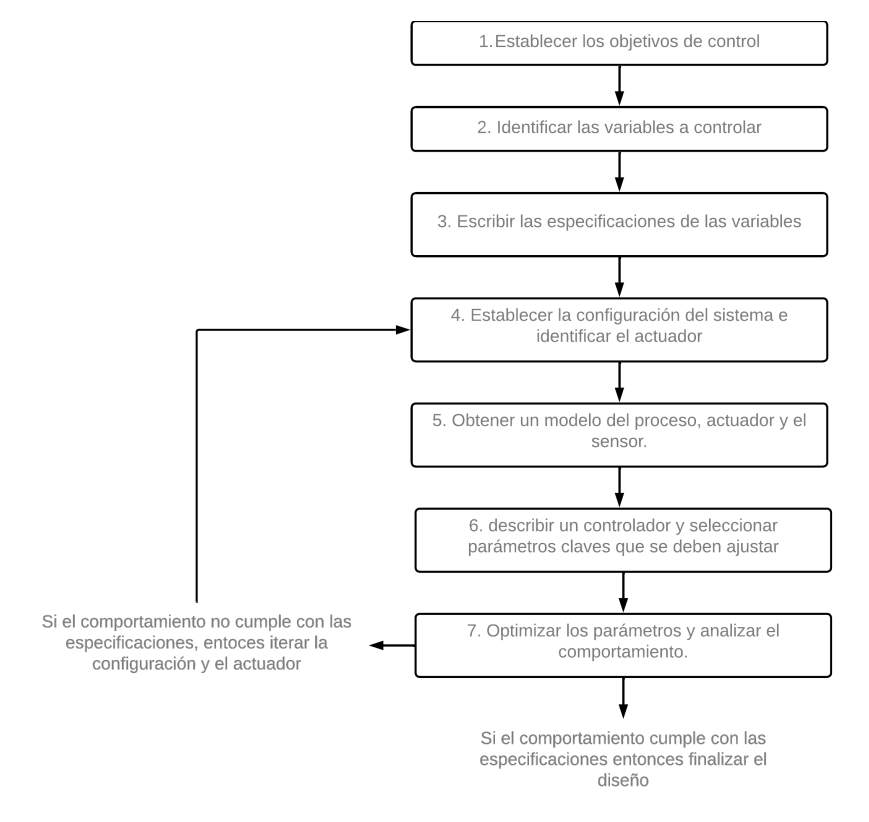
\includegraphics[scale=0.5]{diagramas/image.png}
  \caption{Proceso de diseño para el control de un sistema Fuente: \cite{4}}
  \label{fig:diagrama}
\end{figure}


%% Hablar de open API

Por otro lado, los modelos de programación en la actualidad cuentan con grandes conjuntos de herramientas, bibliotecas, frameworks entre otros los cuales han sido desarrollados para facilitar la programación de software, además algunas de ellas están desarrolladas para proporcionar un sistema unificados de programación que permita que los desarrolladores aprovechen de forma más eficiente los recursos de hardware heterogéneos. Esto se refiere a entornos informáticos los cuales utilizan distintos componentes de hardware con el fin de mejorara el rendimiento y la eficiencia de ejecución de tareas especificas, estos se pueden encontrar como Unidades de procesamiento central (CPUs), Unidades de procesamiento gráfico(GPUs), Unidades de procesamiento Tensor(TPUs), Procesadores de señal digital (DSP) entre otros \cite{costanzo2022migrating}.

Un software agnóstico de hardware se puede entender como un programa o aplicación el cual se diseña para funcionar de forma independiente del hardware especifico en el cual se ejecuta, es decir el software se diseña para que el mismo sea compatible con diferentes plataformas sin depender de características o especificaciones de algún hardware. Esta característica es beneficiosa ya que permite a los  hacer uso del mismo en una variedad de equipo sin preocuparse por la compatibilidad del hardware\cite{nozal2021exploiting}.

Algunos de estos modelos de programación se encuentran bajo el nombre de NVIDIA CUDA, OpenCL, AMD ROCm, Intel OneAPI entre otras y se caracterizan por todas ser frameworks de programación y plataformas para facilitar la computación paralela en diferentes tipos de hardware, por lo general GPUs y otros aceleradores.
\newpage

\section{Definición del problema}

\subsection{Generalidades}

%Describe la necesidad de un sistema de control eficiente en el entorno actual.
Los sistemas de control siempre dependen de un proceso de caracterización del proceso físico, es decir, estos se basan en un modelo matemático dependiente del tiempo, el mismo deberá de representar la dinámica de la planta  y el sistema debe de contar con al menos un actuador y un sensor, esto con el fin de leer datos y realimentar el sistema. Eso se puede obtener de forma teórica mediante el modelado de la planta o bien de forma empírica en la cual se toman los datos de forma directa de la planta y la misma se somete a un impulso conocido esto con el fin de lograr determinar el comportamiento de la misma ante el estimulo ingresado a la misma, de esto se parte al estudio de los datos de entrada y salida, el proceso es conocido como identificación. Una de las ventajas de la forma empírica es que mediante la toma de datos de la planta se pueden ingresar pequeñas perturbaciones manuales a la planta en cuestión con el objetivo de observar a nivel de datos el comportamiento de la misma \cite{15-tec}. 

Con la presencia de las no linealidades en algunos sistemas de control y que no todos los sistemas son compuestos por una entrada y una salida se vuelve mas complejo la descripción del sistema  de control y por ende se requiere una mayor cantidad de ecuaciones, haciendo que cada vez según avancen los sistemas de control los mismo sean mas difíciles de derivar para que los sistemas logren un equilibrio aceptable entre precisión y velocidad de respuesta, además que sin importar que existan métodos clásicos estos no siempre van a conducir a resultados aceptados. Esto dificulta el procesos e obtención de un modelo matemático representativo para el sistema. Ahora bien la mayor parte de sistemas que se encuentran en la naturaleza son no lineales y los sistemas que son aplicados a solucione modernas de ingeniera tienden a presentar problemas de control , tales como los sistemas de comando de vuelo que presentan como mínimo 6 entradas y 4 salidas, es acá donde se torna de gran importancia un método o técnica de control el cual permita identificar y controlar el sistema \cite{15-tec}. 

%Explica el propósito de diseñar e implementar un software agnóstico de hardware

Por otro lado un software agnóstico de hardware es un sistema el cual esta diseñado para gestionar y controlar proceso sin depender de un hardware en especial, estos son caracterizados por presentar una compatibilidad con diversos dispositivos lo que permite al usuario final hacer uso del sistema en distintos entornos de hardware sin la necesidad de generar modificaciones significativas al entorno original, también es un sistema el cual se basa en estándares industriales y hace uso de protocolos de comunicación comunes, esto con el fin de facilitar la integración con dispositivos normalizados, permitiendo, de esta forma la configuración de parámetros según el hardware en el cual se ejecute y de esta forma se pretende garantizar que el software optimice su rendimiento según las capacidades de los dispositivos deseados\cite{krainiuk2021oneapi}. 

Finalmente se debe de tomar en cuenta que una de las peculiaridades de los software agnóstico de hardware es sacar provecho a las cualidades que presentan para la automatización de procesos esto con el fin de programar tareas especificas, toma de decisiones y ajustar la información de salida respecto a una entrada que reciba el sistema, no sin dejar por fuera que implementa una capa de abstracción la cual es encargada de ocultar detalles específicos del hardware, permitiendo al software centrarse solamente en la lógica de control sin importar los detalles del entorno. En síntesis es un sistema el cual busca ser versátil, ínter-operable y fácilmente adaptable a distintos entornos y dispositivos sin requerir modificaciones en el código fuente.


\subsection{Síntesis del problema}

En la Escuela de Ingeniería Electrónica y el SIPLab, se ha identificado una carencia a nivel de implementación de un sistema de control automático, el cual funcione de la misma forma independientemente del  hardware al cual se conecte y que además de esto simplifique la configuración de parámetros de operación deseados, ya que actualmente limita los procesos de enseñanza tanto en las ares de aprendizaje automático como en control.

%En la Escuela de Ingeniería Electrónica y el SIPLab, se ha observado una gran carencia a nivel de implementación cuanto a técnicas de control automático capaces de lidiar con volúmenes de operación no han sido explorados, lo cual limita los procesos de enseñanza tanto en las ares de aprendizaje automático como en control.


%En la Escuela de Ingeniería Electrónica y el SIPLab, se ha identificado una carencia en la exploración de técnicas de control automático capaces de gestionar volúmenes de operación. Esta falta de investigación limita el avance en los procesos de enseñanza, especialmente en las áreas de aprendizaje automático y control.

\section{Enfoque de la solución}

Como se menciono en el apartado de definición del problema la implementación de un software agnóstico de hardware como interfaz de comunicación entre el usuario y la planta a controlar presenta la eliminación de muchas dependencias además de permitir una portabilidad del controlador a cualquier plataforma de hardware que posea entradas y salidas programables. Es por esto que a continuación se proponen tres alternativas de implementación para el control de una planta prototipo no lineal en todo su espacio de operación mediante técnicas de control automático que el SIPLab ha investigado en el ultimo año. La planta seleccionada para la implementación del esta interfaz sera la planta de péndulo amortiguado a hélice (PAHM). Además de esto se propone utilizar un sistema embebido de altas prestaciones que sea capaz de ejecutar el programa, lo que a su vez impone limitaciones a la complejidad del algoritmo a seleccionar.

Finalmente, basándonos en matriz de Pugh se analizan las soluciones con el objetivo de seleccionar la solución mas adecuada, en donde un cero indica que la alternativa es similar, un +1 que la alternativa es mejor y un -1 que la alternativa es peor en el criterio comparada a la referencia.

\subsection{Alternativa 1}

Como primer alternativa de solución se propone hacer uso de técnicas de control adaptativo, técnica que da sus comienzos en la década de los 80, aunque existían limitaciones tecnológicas que hacían que esta alternativa fuera muy costosa. Actualmente,
no está sujeto a esas limitaciones, pues se puede desarrollar esta técnica a bajo costo y con un procesamiento alto y rápido\cite{15-tec}.

El control adaptativo busca mejorar el funcionamiento de la planta modificando su comportamiento en respuesta a los cambios en la dinámica del sistema y a perturbaciones externas, que con el tiempo deterioran su funcionamiento. Además, este permite realizar ajustes al controlador en tiempo real. Esto se realiza utilizando técnicas que miden las variables dinámicas de la planta de forma continua, las compara con parámetros deseados y mediante su diferencia modifica las características del controlador, generando así un accionamiento que mantiene las variables de la planta en un rango de desempeño\cite{15-tec}.

Se haría uso de un filtro de Kalman para la estimación de parámetros o variables de estado cuando el sistema presenta ruidos aditivos. Además, este filtro proporciona una predicción del estado futuro del sistema, basado en estimaciones pasadas, lo que ayuda al controlador adaptativo a adaptarse de mejor forma ante problemas o perturbaciones que ocurran en el sistema\cite{15-tec}.

\subsection{Alternativa 2}

Como segunda alternativa se propone hacer uso de aprendizaje automático para llevar a cabo el control de la PAHM, esto mediante el uso de redes neuronales artificiales ya que una de las principales características de estas mismas es el aprendizaje de relaciones complejas a partir de un conjunto de ejemplos. Además de esto debido a sus capacidades de aproximación y adaptabilidad las RNA presentan una muy buena alternativa en el modelado de sistemas no lineales y en la comprensión de los mismos. Como una alternativa a los controladores clásicos es ofrecido en el caso del aprendizaje reforzado RL, el cual ofrece algunos algoritmos para el desarrollo de controladores óptimos de sistemas con dinámicas no lineales\cite{15-tec}. 

Estos algoritmos mencionados anteriormente operan bajo la metodología la cual tiene como objetivo que un agente sea capaz de encontrar la acción correcta de manera autónoma, explorando un espacio desconocido y determinando la acción mediante prueba y error ya que estos sistemas aprenden por medio de la aplicación de recompensas y penalizaciones las cuales obtienen mediante sus acciones, esto con el objetivo de crear la mejor estrategia posible. Cabe destacar que esta metodología se ha aplicado en otros sistemas de control en donde no basta con la aplicación de las técnicas de control clásicas. Permitiendo de esta forma automatizar el proceso mas allá de lo alcanzable con los métodos tradicionales\cite{naizhang2022intel}. 

Por otro el uso de software agnóstico de hardware ofrece una gran versatilidad ya que sus características permiten la ejecución del mismo en una gran variedad de dispositivos , lo cual a nivel de plataforma resulta en elegir el hardware según las necesidades sin preocuparse por la compatibilidad del software, también se debe de tomar en cuenta que las dependencias a nivel de hardware son menores ya que al no depender de una configuración de hardware como tal reduce la dependencia a nivel de marcas o modelos, lo cual permite una fácil migración a distintos dispositivos sin perder la funcionalidad. Finalmente se puede hacer referencia a una compatibilidad a largo plazo ya que el software no se encuentra atado a alguna generación especifica\cite{krainiuk2021oneapi}. 


\subsection{Alternativa 3}

La tercera alternativa de solución es similar a lo planteado en la anterior, ya que también hace uso de una red neuronal artificial basada en aprendizaje reforzado para controlar la planta PAHM, debido a su facilidad de aproximación, su adaptabilidad y demás características anteriormente expuestas. Lo que hace diferente a esta alternativa, es la aplicación de una única red neuronal directamente sobre la planta PAHM\cite{15-tec}.

\subsection{Selección de la solución}

Una vez contempladas las bondades que ofrecen las 3 alternativas el criterio de desciño se basa en los resultados obtenidos mediante la generación de la matriz de Pugh la cual se puede observar en la Tabla 1.

\begin{figure}[h]
  \centering
  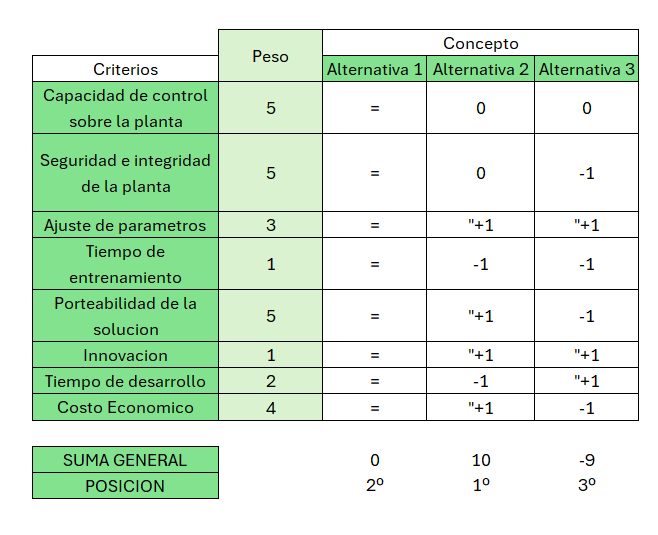
\includegraphics[scale=0.7]{tablas/pugh.png}
  \captionsetup{labelformat=empty}  % Eliminar la etiqueta predeterminada ("Figura")
  \caption{Tabla 1: Matriz de Pugh para la selección de la solución}
\end{figure}

Cuando se realiza el análisis de la Matriz de Pugh se puede determinar que en aspectos como lo son ajustes de parámetros o innovación la Alternativa 2 y 3 se encuentran empatadas ya que hay que recordar que lo que difiere entre estas dos opciones es el método de implementación, por un lado en la Alternativa 2 se propone el uso de un software agnóstico de Hardware como base del diseño mientras que en la Alternativa 3 se plantea el uso de un método mas tradicional y dependiente del hardware, eliminando virtudes de la alternativa 2 como lo era la portabilidad de la solución a otros sistemas de control sin importar sobre el hardware que se ejecutara el mismo. Es por esto que criterios como lo fueron el costo económico terminaron de inclinar la balanza por el uso de la Alternativa 2. 

\section{Meta}

Controlar exitosamente la planta prototipo utilizando aprendizaje reforzado, estabilizando el sistema en un rango de tiempo máximo del 10 \% del control clásico, con un sobre impulso inferior al 5 \%, cero error de estado estacionario y la reducción de perturbaciones de entrada o salida a la planta.

\section{Objetivo General}

Desarrollar un programa que logre controlar el comportamiento dinámico de una planta prototipo mediante el uso de redes neuronales independientemente del hardware en el cual se ejecute el mismo.

\textbf{Indicador:} La red neuronal controla a la planta PAHM de movimiento dinámico, en donde la respuesta a una determinada entrada ingresada posee un porcentaje de error inferior al 10\%.

\section{Objetivos Específicos}

\begin{enumerate}
    \item Lograr que la Gated Recurrent Unit (GRU) generada posteriormente en este proyecto funcione en tiempo real.\newline
    \textbf{Indicador:} Se deberá de adaptar la paramtrizacion de los datos de entrada para que el sistema logre interpretarlos en tiempo real, esto haciendo uso del sistema dinámico a controlar.
    
    \item Seleccionar el algoritmo de RL para controlar la planta.\newline
    \textbf{Indicador:} Se define como control de la planta que la misma llegue a un ángulo deseado y que la planta intente llegar ahí lo más rápido posible, con el menor sobre impulso posible.  


    \item Investigar sobre los  entorno de desarrollo que permiten la generación de software agnóstico de hardware.\newline
    \textbf{Indicador:} Mediante una investigación se deberá de reunir mas información sobre al menos 4 tipos de  entorno de desarrollo que permitan la generación de software agnóstico de hardware.

    \item Generar programas de prueba en distintos lenguajes de programación los cuales permitan identificar la compatibilidad de los  entorno de desarrollo con los sistemas a controlar.\newline
    \textbf{Indicador:} Se generaran programas de prueba con el fin de evaluar mediante indicadores y métricas de desempeño la eficiencia del sistema, esto con el fin de encontrar el lenguaje de programación óptimo que ingrese la menor cantidad de retraso al procesamiento de las señales.

    \item Evaluar la respuesta del programa generado utilizando la red neuronal artificial mimetizadora como entrada del sistema.\newline
    \textbf{Indicador:} Mediante métricas de desempeño y simulaciones se pondrá a prueba la respuesta del sistema ante el comportamiento dinámico de la planta para una entrada determinada.

    \item Evaluar la respuesta del programa generado utilizando la planta de control PAHM como entrada del sistema.\newline
    \textbf{Indicador:} Mediante el uso de métricas y simulaciones se comparara el funcionamiento de la PAMH siendo controlada por el programa generado y un control tradicional.
\end{enumerate}

\section{Procedimiento para la ejecución del proyecto}

Sobre la ejecución del proyecto se planifican las actividades de forma jerárquica, en donde se establecen actividades según los objetivos planteados, los requisitos de las actividades y la dependencia que tenga este mismo con alguna actividad previa. Además de esto se definen los tiempos de duración de las actividades las cuales se resumen en la Tabla 2.

\begin{figure}[h]
  \centering
  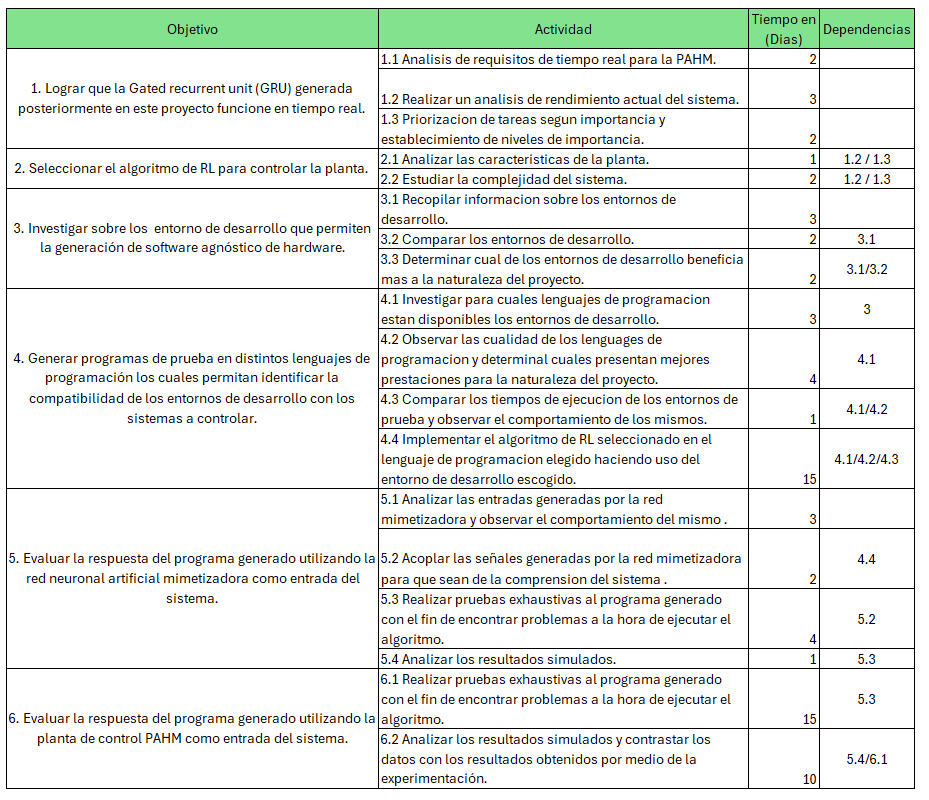
\includegraphics[scale=0.6]{tablas/ejecucion.png}
  \captionsetup{labelformat=empty}  % Eliminar la etiqueta predeterminada ("Figura")
  \caption{Tabla 2: Procedimientos para la ejecución del proyecto}
\end{figure}

\section{Cronograma de actividades}

La agenda de actividades según el tiempo asignado comprende desde el xxx de Febrero del 2024 hasta el xxx de Mayo del 2024, tiempo el cual abarca 16 semanas lectivas en las cuales se llevara a cabo el desarrollo del proyecto. Por un lado el cronograma se presenta como un diagrama de Gantt, el mismo se puede observar en la Figura \ref{fig:gantt}. Por otro lado en la Figura \ref{fig:pert} se muestra el diagrama de PERT para lograr observar de una forma mas sencilla la dependencia entre actividades.


\begin{figure}
  \centering
  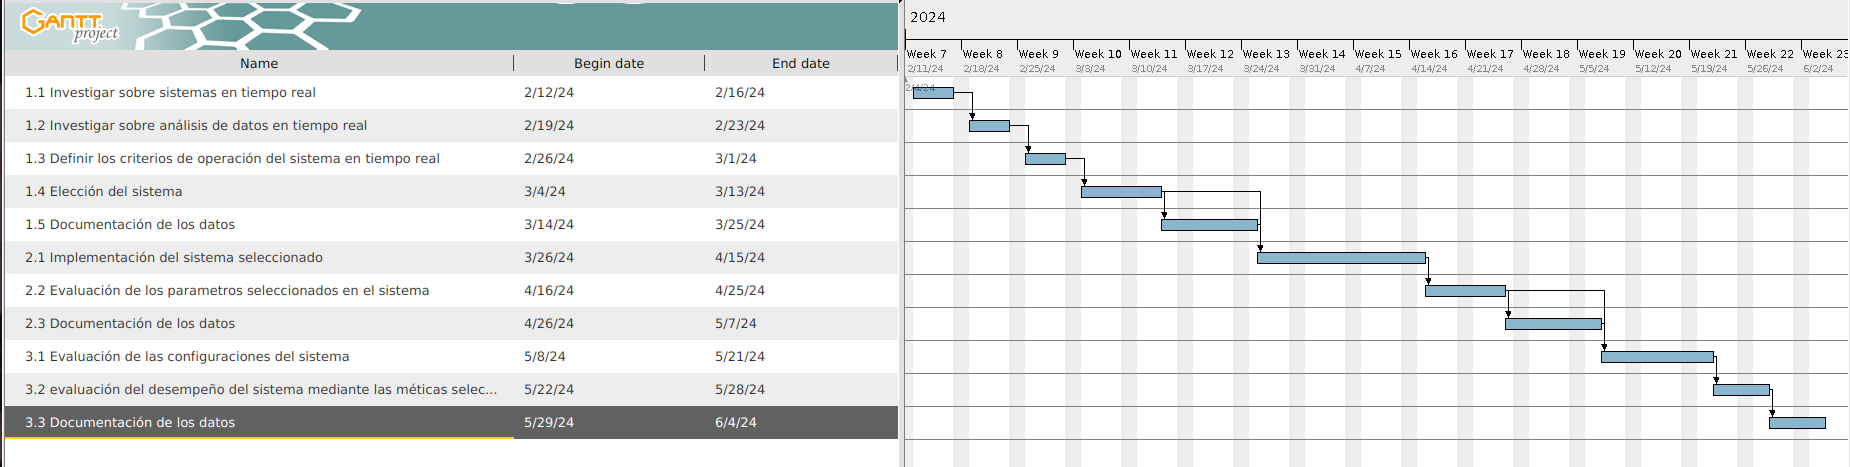
\includegraphics[scale=0.3, angle=90]{diagramas/gantt.png}
  \caption{Ruta critica del cronograma de actividades}
  \label{fig:gantt}
\end{figure}

\begin{figure}
  \centering
  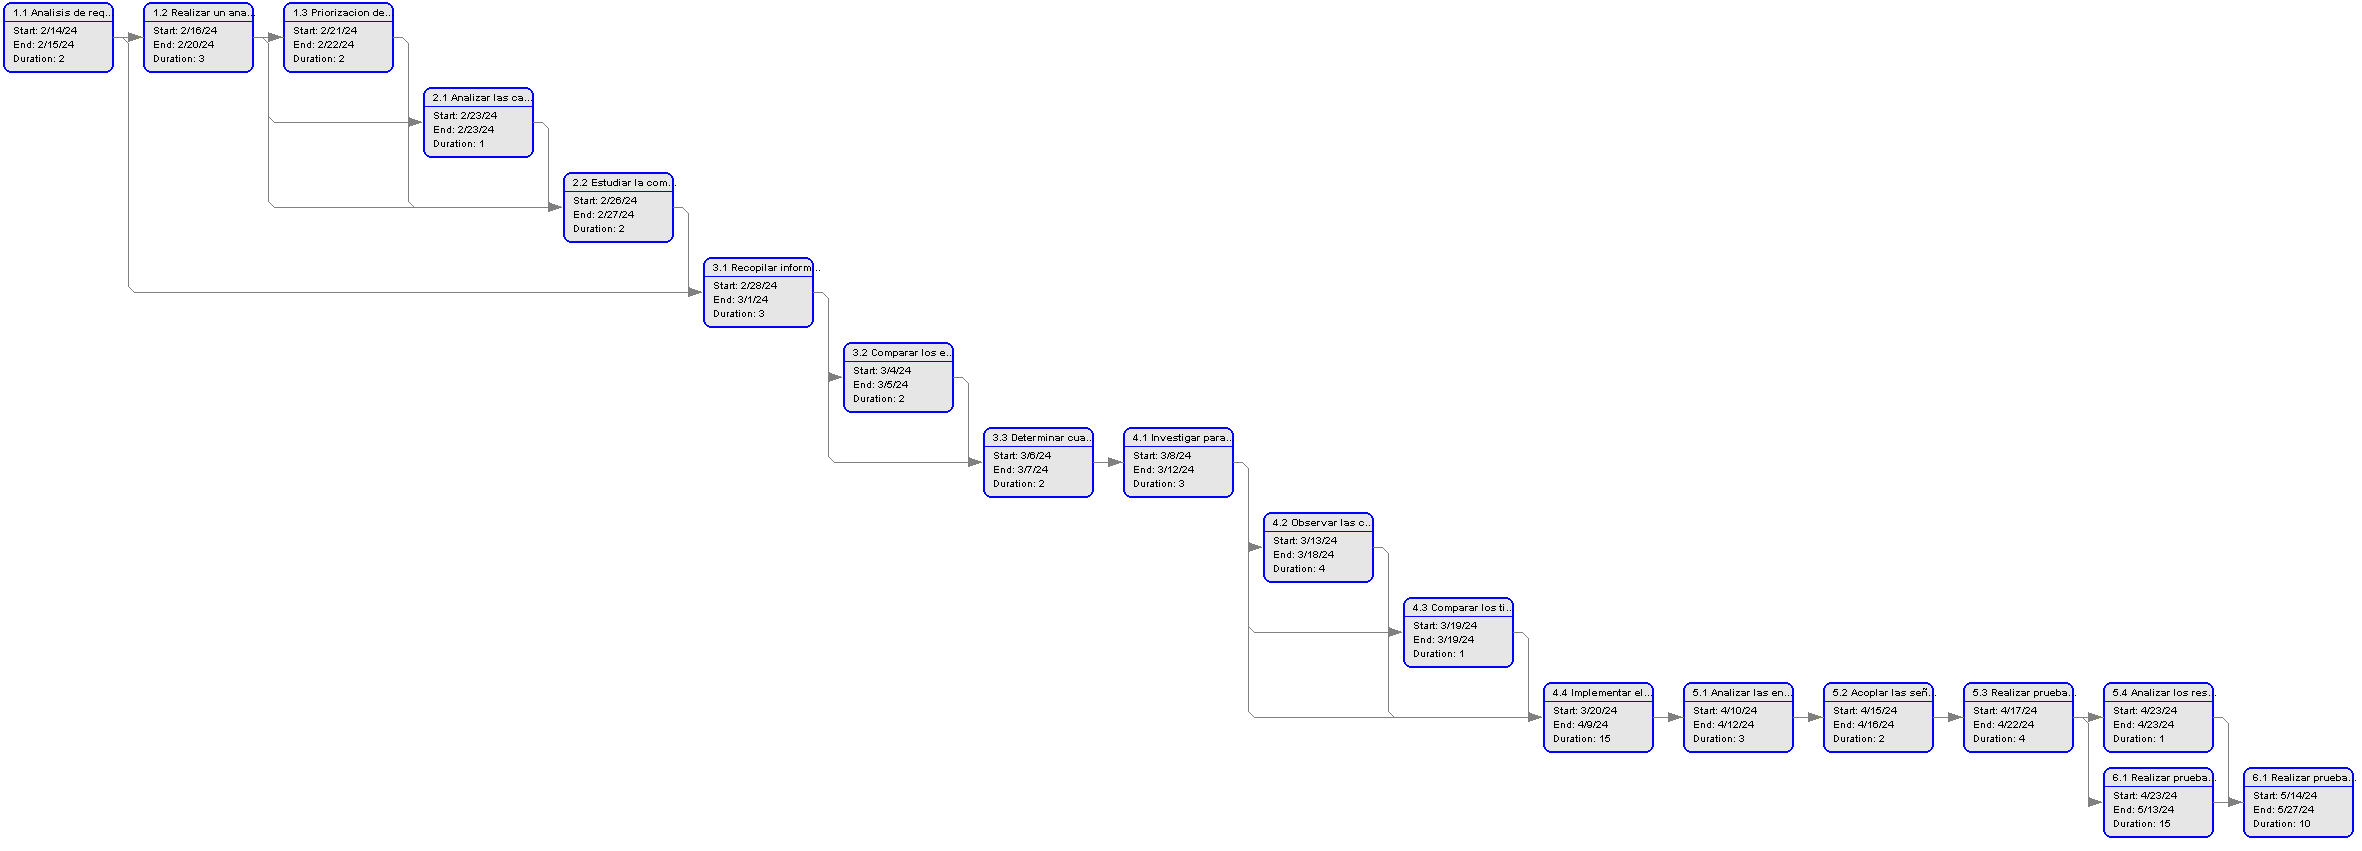
\includegraphics[scale=0.3, angle=90]{diagramas/pert.png}
  \caption{Diagrama PERT de las actividades}
  \label{fig:pert}
\end{figure}


\subsection{Entregables}

Como se puede observar en la Tabla 3 se encuentra una lista de los entregables con sus objetivos y fechas de entrega establecidas en el periodo donde se llevara a cabo el trabajo final de graduación.

\begin{figure}[h]
  \centering
  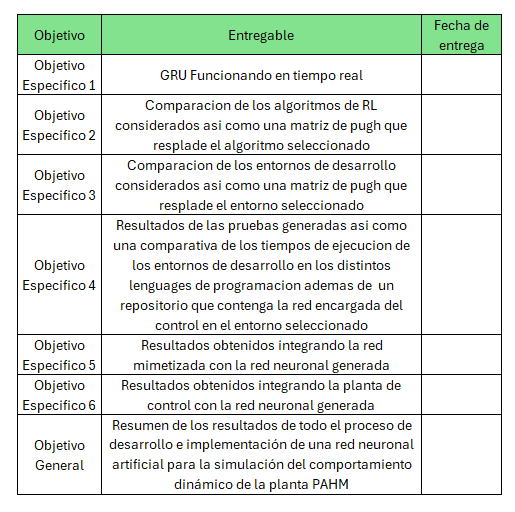
\includegraphics[width=0.6\textwidth]{tablas/entregable.png}
  \captionsetup{labelformat=empty}  % Eliminar la etiqueta predeterminada ("Figura")
  \caption{Tabla 3: Lista de entregables}
\end{figure}

\section{Uso de recursos}

Para ejecutar el software encargado de controlar la planta prototipo por medio de aprendizaje reforzado se hace uso de la siguiente lista de materiales.

\begin{itemize}
    \item Una planta prototipo de control automático donde se implemente el controlador.
    \item Computadora donde desarrollar el controlador. En caso de ser portátil, se requiere accesorios como el cargador.
    \item Tarjeta de desarrollo NVIDIA Jetson TX2.
    \item Acceso a internet para llevar a cabo las revisión bibliográfica.
    \item Tiempo de cómputo para el entrenamiento de las redes neuronales
\end{itemize}

\newpage

\section{Presupuesto}

\begin{figure}[h]
  \centering
  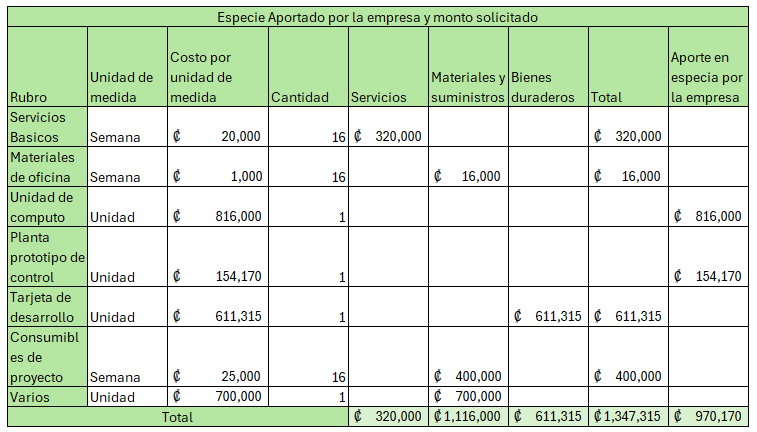
\includegraphics[scale=0.8]{tablas/ptot.png}
  \captionsetup{labelformat=empty}  % Eliminar la etiqueta predeterminada ("Figura")
  \caption{Tabla 4: Presupuesto para realizar el proyecto}
\end{figure}

\begin{figure}[h]
  \centering
  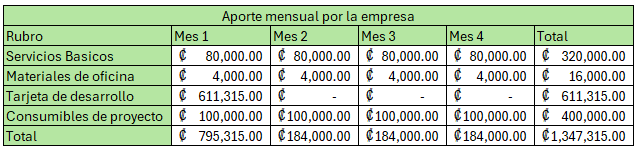
\includegraphics[scale=0.8]{tablas/pmensual.png}
  \captionsetup{labelformat=empty}  % Eliminar la etiqueta predeterminada ("Figura")
  \caption{Tabla 5: Presupuesto Mensual para realizar el proyecto}
\end{figure}

\newpage
\renewcommand{\refname}{Bibliografía}
\bibliography{biblio}
\nocite{*}
\bibliographystyle{plain}

\end{document}
